\documentclass[a4paper,twoside]{article}
\usepackage{blindtext}  
\usepackage{geometry}

% Chinese support
\usepackage[UTF8, scheme = plain]{ctex}

% Page margin layout
\geometry{left=2.3cm,right=2cm,top=2.5cm,bottom=2.0cm}


\usepackage{listings}
\usepackage{xcolor}
\usepackage{geometry}
\usepackage{amsmath}
\usepackage{float}
\usepackage{hyperref}

\usepackage{graphics}
\usepackage{graphicx}
\usepackage{subcaption}
\usepackage{epsfig}
\usepackage{float}

\usepackage{algorithm}
\usepackage[noend]{algpseudocode}

\usepackage{booktabs}
\usepackage{threeparttable}
\usepackage{longtable}
\usepackage{tikz}
\usepackage{multicol}

% cite package, to clean up citations in the main text. Do not remove.
\usepackage{cite}

\usepackage{color,xcolor}

%% The amssymb package provides various useful mathematical symbols
\usepackage{amssymb}
%% The amsthm package provides extended theorem environments
\usepackage{amsthm}
\usepackage{amsfonts}
\usepackage{enumerate}
\usepackage{enumitem}
\usepackage{listings}
\usepackage{minted}


\usepackage{indentfirst}
\setlength{\parindent}{2em} % Make two letter space in the first paragraph
\usepackage{setspace}
\linespread{1.5} % Line spacing setting
\usepackage{siunitx}
\setlength{\parskip}{0.5em} % Paragraph spacing setting

% \usepackage[contents =22920202204622, scale = 10, color = black, angle = 50, opacity = .10]{background}

\renewcommand{\figurename}{图}
\renewcommand{\listingscaption}{代码}
\renewcommand{\tablename}{表格}
\renewcommand{\contentsname}{目录}
\floatname{algorithm}{算法}

\graphicspath{ {images/} }

%%%%%%%%%%%%%
\newcommand{\StudentNumber}{22920202204622}  % Fill your student number here
\newcommand{\StudentName}{熊恪峥}  % Replace your name here
\newcommand{\PaperTitle}{实验(五)中间代码生成器}  % Change your paper title here
\newcommand{\PaperType}{编译原理} % Replace the type of your report here
\newcommand{\Date}{2023年6月5日}
\newcommand{\College}{信息学院}
\newcommand{\CourseName}{编译原理}
%%%%%%%%%%%%%

%% Page header and footer setting
\usepackage{fancyhdr}
\usepackage{lastpage}
\pagestyle{fancy}
\fancyhf{}
% This requires the document to be twoside
\fancyhead[LO]{\texttt{\StudentName }}
\fancyhead[LE]{\texttt{\StudentNumber}}
\fancyhead[C]{\texttt{\PaperTitle }}
\fancyhead[R]{\texttt{第{\thepage}页,共\pageref*{LastPage}页}}


\title{\PaperTitle}
\author{\StudentName}
\date{\Date}

\algnewcommand\algorithmicinput{\textbf{Input:}}
\algnewcommand\algorithmicoutput{\textbf{Output:}}
\algnewcommand\Input{\item[\algorithmicinput]}%
\algnewcommand\Output{\item[\algorithmicoutput]}%

\newenvironment{longlisting}{\captionsetup{type=figure}}{}

\usetikzlibrary{positioning, shapes.geometric}

\begin{document}
	
%%%%%%%%%%%%%%%%%%%%%%%%%%%%%%%%%%%%%%%%%%%%
\makeatletter % change default title style
\renewcommand*\maketitle{%
	\begin{center} 
		\bfseries  % title 
		{\LARGE \@title \par}  % LARGE typesetting
		\vskip 1em  %  margin 1em
		{\global\let\author\@empty}  % no author information
		{\global\let\date\@empty}  % no date
		\thispagestyle{empty}   %  empty page style
	\end{center}%
	\setcounter{footnote}{0}%
}
\makeatother
%%%%%%%%%%%%%%%%%%%%%%%%%%%%%%%%%%%%%%%%%%%%
	
	
\thispagestyle{empty}

\vspace*{1cm}

\begin{figure}[htb]
	\centering
	
\includegraphics[width=4.0cm]{logo.png}
\end{figure}

\vspace*{1cm}

\begin{center}
	\Huge{\textbf{\PaperType}}
	
	\Large{\PaperTitle}
\end{center}

\vspace*{1cm}

\begin{table}[H]
	\centering	
	\begin{Large}
		\renewcommand{\arraystretch}{1.5}
		\begin{tabular}{p{3cm} p{5cm}<{\centering}}
			姓\qquad 名 & \StudentName  \\
			\hline
			学\qquad号 & \StudentNumber \\
			\hline
			日\qquad期 & \Date  \\
			\hline
			学\qquad院 & \College  \\
			\hline
			课程名称 & \CourseName  \\
			\hline
		\end{tabular}
	\end{Large}
\end{table}

\newpage

\title{
	\Large{\textcolor{black}{\PaperTitle}}
}
	
	
\maketitle
	
\tableofcontents
 
\newpage
\setcounter{page}{1}

\begin{spacing}{1.2}

\section{实验目的}

掌握中间代码生成器的构造原理和编程方法。

\section{实验内容}

用自顶向下方法或Yacc进行语法分析的基础上,编写一个中间代码生成程序。

\section{运行结果}

运行结果如图~\ref{fig:output},该程序会在控制台输出结果的同时,将结果写入\texttt{generate.txt}中。
完整输出内容见\nameref{sec:fullout}。
\begin{figure}[htb]
	\centering
	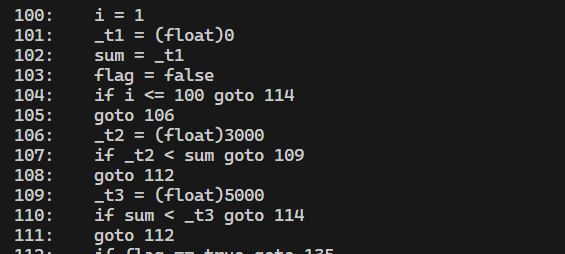
\includegraphics[width=0.6\linewidth]{output.png}
	\caption{运行结果}
	\label{fig:output}
\end{figure}


\section{支持break}

为了支持\texttt{break},程序需要进行以下的操作:
\begin{itemize}
	\item 检查\texttt{break}是否在循环中,如果不在循环中,则报错。
	\item 生成一条中间代码,跳转到正确的位置。
\end{itemize}

考虑到循环天然具有嵌套的特性,因此自然地可以使用栈来记录当前是否在循环中。为了能够正确入栈,
考虑到YACC采取的是自底向上的分析方法,因此需要在\texttt{for}和\texttt{while}的产生式中加入一个空产生式$Q\rightarrow\epsilon$进行入栈操作。

空产生式$Q\rightarrow\epsilon$的动作中,程序会执行如下操作:
\inputminted[firstline=90,lastline=91]{c}{../code/grammar.y}
\texttt{break\_lists}是用于记录\texttt{break}位置同时反映嵌套循环的栈。在$Q$产生式被使用时,程序会将\texttt{break\_lists}中入栈一新的元素,等待后续的产生式
将其设为正确的\texttt{break}位置。
进而,循环语句$DO$和$WHILE$的产生式也需要分别修改成$stmt\rightarrow \ DO \ Q \ M \ stmt \ldots$和$stmt\rightarrow \ WHILE \ Q \ M \ldots$。
这样一来,使用这些产生式进行分析时就会导致$Q$被使用。

在循环结束后,程序会将栈顶出栈,然后加入循环的$nextlist$中。这样一来,就可以和其他产生式一起正确地生成中间代码了。

在入栈出栈操作之外,程序还需要在\texttt{break}的产生式中生成一个\texttt{goto}中间代码,它负责跳转到正确的位置。
由于\texttt{break}的产生式中,\texttt{break}的位置已经被记录在\texttt{break\_lists}栈中,
然后栈顶又会加入到循环的$nextlist$中,因此这条\texttt{goto}中间代码的位置也会在进行回填时被一同正确地确定,无需进一步额外处理。

以\texttt{while}循环为例,处理它的动作如下:
\inputminted[firstline=118,lastline=124]{c}{../code/grammar.y}
而\texttt{break}的动作如下:
\inputminted[firstline=131,lastline=141]{c}{../code/grammar.y}
这些动作完全实现了上述逻辑。其中\texttt{merge\_goto\_list}是额外实现的一个函数,它的作用是将两个链表合并成一个。


\section{实验总结}

在本次实验中,我通过在基于YACC的语法分析器上进一步实现一个中间代码生成器,进一步加深了对编译原理的理解。
同时,也加深了对中间代码生成一章中的知识的体会,更深刻地理解了书中所给出的翻译方案,并亲自动手实现了它们。

这是本学期最后一次实验,在本学期的实验中,我从词法分析器开始,逐步从手写的词法分析器过渡到基于LEX的词法分析器,然后再到基于YACC的语法分析器,
最后,综合以上学习到的工具,以及语法制导定义、语法制导翻译方案的各项知识,综合应用完成了此次中间代码生成器的实验。
虽然在实验过程中遇到了一些困难,但是在实验中,我学习到了如何使用工具生成编译器,更获得了将理论知识应用到实践中的经验。

虽然以前有过实现编译器的经验,但是经过一学期的课程,我将自学的、碎片化的知识系统化、完善化,同时也学会了很多新的知识,
例如在实践过程中被我忽略的自底向上的语法分析,以及在实践中一直在使用,但是没有系统、全面认识的语法制导定义、语法制导翻译方案等等。
在一学期的过程中,我应用了大学三年以来学习到的几乎所有知识来完成实验,又对照我以前的经验,进行进一步的总结、提升和修正。
这一学期的实验和理论学习确实让我受益匪浅,收获颇丰。

最后,感谢老师和助教老师们一学期以来的答疑解惑和辛苦付出!

\clearpage
\appendix
\section{附录:完整输出}
\label{sec:fullout}

\inputminted{bnf}{text/generate.txt}


\end{spacing}

\end{document}